\begin{figure}
\centering
\begin{subfigure}[b]{0.49\textwidth}
    \centering
    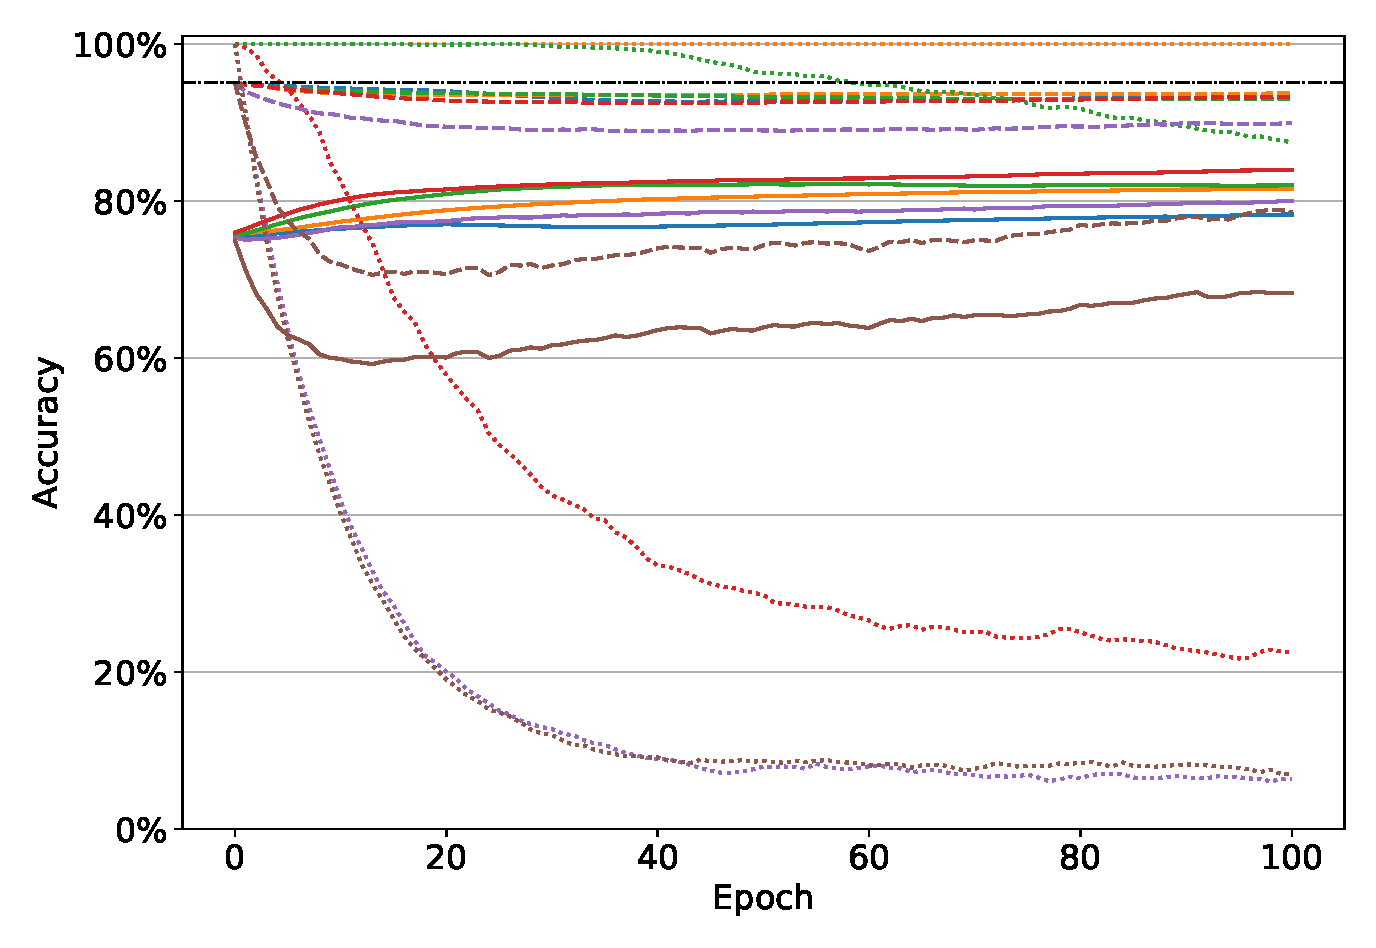
\includegraphics[width=\linewidth]{images/finetuning/finetuning_protecting_content_smoothed_imagenet_0.eps}
    \caption{Fine-Tuning on CINIC-10}
    \label{fig:fine-tuning-cinic10}
\end{subfigure}
\begin{subfigure}[b]{0.49\textwidth}
    \centering
    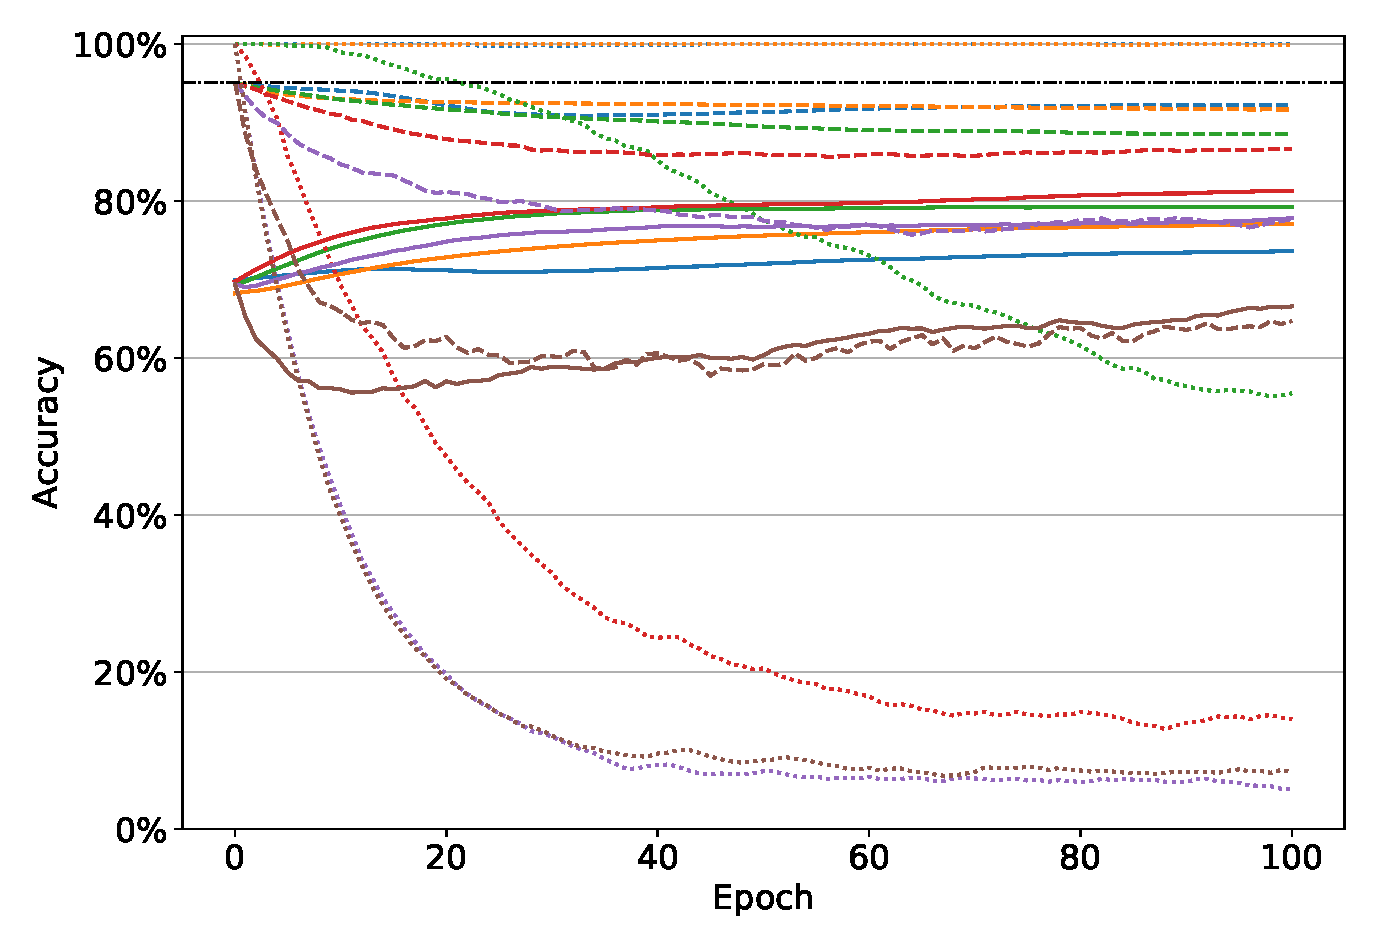
\includegraphics[width=\linewidth]{images/finetuning/finetuning_protecting_content_smoothed_imagenet_1.eps}
    \caption{Fine-Tuning on ImageNet part of CINIC-10}
    \label{fig:fine-tuning-cinic10-imagenet}
\end{subfigure}

\begin{subfigure}[b]{\linewidth}
    \centering
    \includegraphics[height=1.1cm]{images/finetuning/legend_content_finetuning_imagenet_colors.eps}
    \quad
    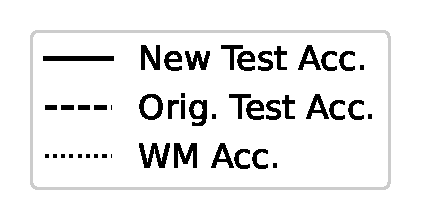
\includegraphics[height=1.1cm]{images/finetuning/legend_content_finetuning_imagenet_linetypes.eps}
\end{subfigure}

\caption{Fine-Tuning on both, CINIC-10 and only on the ImageNet part of CINIC-10. In both cases, 50,000 images are randomly chosen from the corresponding dataset. The underlying model is a ResNet-18 that was trained with \textit{ProtectingIP-pattern} and 100 trigger images. The black dash-dotted line corresponds to the benchmark test accuracy of the non-watermarked model. For clearity reasons, the lines in the plot are smoothed. The original plots are provided in \cref{fig:fine-tuning-both-cinic10-imagenet-original}.}
\label{fig:fine-tuning-both-cinic10-imagenet}

\end{figure}